\documentclass{standalone}
\usepackage{tikz}
\usetikzlibrary{patterns, positioning}
\usetikzlibrary{shapes.misc}
\usepackage[outline]{contour}
\contourlength{1.5pt} 


\begin{document}
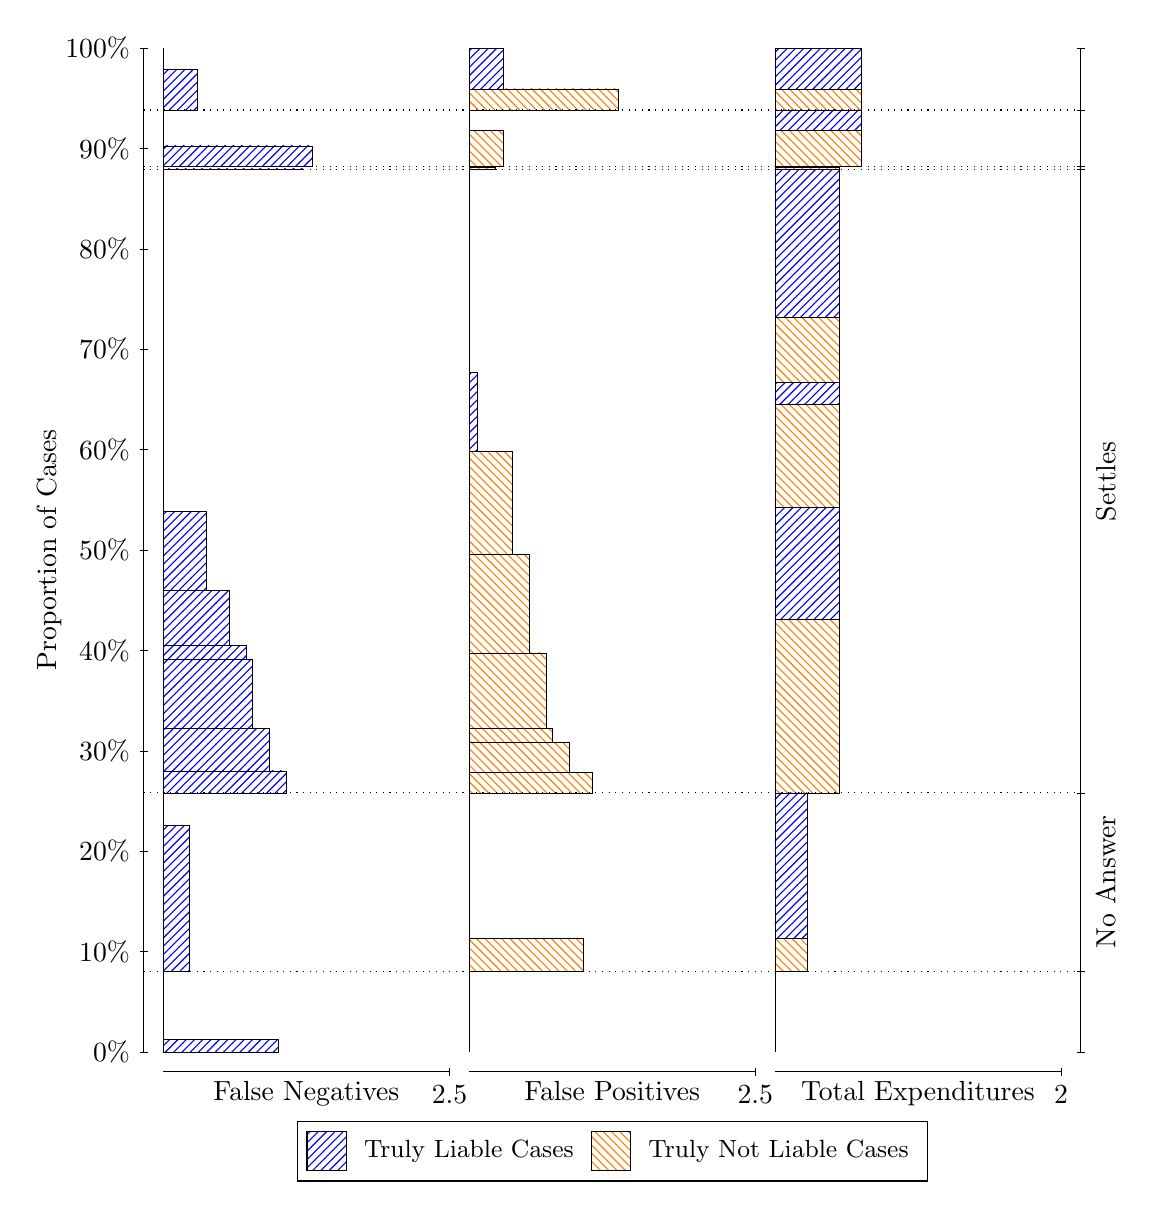
\begin{tikzpicture}
\draw[black, very thin] (1.5,1.75) -- (1.5,14.5);
\node[rotate=90, text=black, anchor=center] at (0.3, 8.125) {Proportion of Cases};
\draw[black, very thin] (1.45,1.75) -- (1.55,1.75);
\node[text=black, anchor=east] at (1.45, 1.75) {0\%};
\draw[black, very thin] (1.45,3.025) -- (1.55,3.025);
\node[text=black, anchor=east] at (1.45, 3.025) {10\%};
\draw[black, very thin] (1.45,4.3) -- (1.55,4.3);
\node[text=black, anchor=east] at (1.45, 4.3) {20\%};
\draw[black, very thin] (1.45,5.575) -- (1.55,5.575);
\node[text=black, anchor=east] at (1.45, 5.575) {30\%};
\draw[black, very thin] (1.45,6.85) -- (1.55,6.85);
\node[text=black, anchor=east] at (1.45, 6.85) {40\%};
\draw[black, very thin] (1.45,8.125) -- (1.55,8.125);
\node[text=black, anchor=east] at (1.45, 8.125) {50\%};
\draw[black, very thin] (1.45,9.4) -- (1.55,9.4);
\node[text=black, anchor=east] at (1.45, 9.4) {60\%};
\draw[black, very thin] (1.45,10.675) -- (1.55,10.675);
\node[text=black, anchor=east] at (1.45, 10.675) {70\%};
\draw[black, very thin] (1.45,11.95) -- (1.55,11.95);
\node[text=black, anchor=east] at (1.45, 11.95) {80\%};
\draw[black, very thin] (1.45,13.225) -- (1.55,13.225);
\node[text=black, anchor=east] at (1.45, 13.225) {90\%};
\draw[black, very thin] (1.45,14.5) -- (1.55,14.5);
\node[text=black, anchor=east] at (1.45, 14.5) {100\%};

\draw[black, very thin] (13.4,1.75) -- (13.4,14.5);
\draw[black, very thin] (13.35,1.75) -- (13.45,1.75);
\node[anchor=west] at (13.35, 1.75) {};
\draw[black, very thin] (13.35,2.7757) -- (13.45,2.7757);
\node[anchor=west] at (13.35, 2.7757) {};
\draw[black, very thin] (13.35,5.0415) -- (13.45,5.0415);
\node[anchor=west] at (13.35, 5.0415) {};
\draw[black, very thin] (13.35,12.956) -- (13.45,12.956);
\node[anchor=west] at (13.35, 12.956) {};
\draw[black, very thin] (13.35,13.001) -- (13.45,13.001);
\node[anchor=west] at (13.35, 13.001) {};
\draw[black, very thin] (13.35,13.713) -- (13.45,13.713);
\node[anchor=west] at (13.35, 13.713) {};
\draw[black, very thin] (13.35,14.5) -- (13.45,14.5);
\node[anchor=west] at (13.35, 14.5) {};

\draw[black, very thin, pattern color=blue, pattern=north east lines] (1.75,1.75) rectangle (3.2033,1.9113);
\draw[black, very thin, pattern color=orange, pattern=north west lines] (1.75,1.9113) rectangle (1.75,2.7757);
\draw[black, very thin, pattern color=blue, pattern=north east lines] (1.75,2.7757) rectangle (2.077,4.6292);
\draw[black, very thin, pattern color=orange, pattern=north west lines] (1.75,4.6292) rectangle (1.75,5.0415);
\draw[black, very thin, pattern color=blue, pattern=north east lines] (1.75,5.0415) rectangle (3.3123,5.3203);
\draw[black, very thin, pattern color=blue, pattern=north east lines] (1.75,5.3203) rectangle (3.0943,5.8581);
\draw[black, very thin, pattern color=blue, pattern=north east lines] (1.75,5.8581) rectangle (2.8763,6.7406);
\draw[black, very thin, pattern color=blue, pattern=north east lines] (1.75,6.7406) rectangle (2.8037,6.9091);
\draw[black, very thin, pattern color=blue, pattern=north east lines] (1.75,6.9091) rectangle (2.5857,7.6143);
\draw[black, very thin, pattern color=blue, pattern=north east lines] (1.75,7.6143) rectangle (2.295,8.6162);
\draw[black, very thin, pattern color=orange, pattern=north west lines] (1.75,8.6162) rectangle (1.75,12.956);
\draw[black, very thin, pattern color=blue, pattern=north east lines] (1.75,12.956) rectangle (3.5303,12.966);
\draw[black, very thin, pattern color=orange, pattern=north west lines] (1.75,12.966) rectangle (1.75,13.001);
\draw[black, very thin, pattern color=blue, pattern=north east lines] (1.75,13.001) rectangle (3.6393,13.257);
\draw[black, very thin, pattern color=orange, pattern=north west lines] (1.75,13.257) rectangle (1.75,13.713);
\draw[black, very thin, pattern color=blue, pattern=north east lines] (1.75,13.713) rectangle (2.186,14.232);
\draw[black, very thin, pattern color=orange, pattern=north west lines] (1.75,14.232) rectangle (1.75,14.5);
\draw[black, very thin, pattern color=orange, pattern=north west lines] (5.6333,1.75) rectangle (5.6333,2.6144);
\draw[black, very thin, pattern color=blue, pattern=north east lines] (5.6333,2.6144) rectangle (5.6333,2.7757);
\draw[black, very thin, pattern color=orange, pattern=north west lines] (5.6333,2.7757) rectangle (7.0867,3.188);
\draw[black, very thin, pattern color=blue, pattern=north east lines] (5.6333,3.188) rectangle (5.6333,5.0415);
\draw[black, very thin, pattern color=orange, pattern=north west lines] (5.6333,5.0415) rectangle (7.1957,5.3018);
\draw[black, very thin, pattern color=orange, pattern=north west lines] (5.6333,5.3018) rectangle (6.905,5.6814);
\draw[black, very thin, pattern color=orange, pattern=north west lines] (5.6333,5.6814) rectangle (6.687,5.8638);
\draw[black, very thin, pattern color=orange, pattern=north west lines] (5.6333,5.8638) rectangle (6.6143,6.8178);
\draw[black, very thin, pattern color=orange, pattern=north west lines] (5.6333,6.8178) rectangle (6.3963,8.0702);
\draw[black, very thin, pattern color=orange, pattern=north west lines] (5.6333,8.0702) rectangle (6.1783,9.3815);
\draw[black, very thin, pattern color=blue, pattern=north east lines] (5.6333,9.3815) rectangle (5.7423,10.383);
\draw[black, very thin, pattern color=blue, pattern=north east lines] (5.6333,10.383) rectangle (5.6333,12.956);
\draw[black, very thin, pattern color=orange, pattern=north west lines] (5.6333,12.956) rectangle (5.9603,12.991);
\draw[black, very thin, pattern color=blue, pattern=north east lines] (5.6333,12.991) rectangle (5.6333,13.001);
\draw[black, very thin, pattern color=orange, pattern=north west lines] (5.6333,13.001) rectangle (6.0693,13.457);
\draw[black, very thin, pattern color=blue, pattern=north east lines] (5.6333,13.457) rectangle (5.6333,13.713);
\draw[black, very thin, pattern color=orange, pattern=north west lines] (5.6333,13.713) rectangle (7.5227,13.98);
\draw[black, very thin, pattern color=blue, pattern=north east lines] (5.6333,13.98) rectangle (6.0693,14.5);
\draw[black, very thin, pattern color=orange, pattern=north west lines] (9.5167,1.75) rectangle (9.5167,2.6144);
\draw[black, very thin, pattern color=blue, pattern=north east lines] (9.5167,2.6144) rectangle (9.5167,2.7757);
\draw[black, very thin, pattern color=orange, pattern=north west lines] (9.5167,2.7757) rectangle (9.9254,3.188);
\draw[black, very thin, pattern color=blue, pattern=north east lines] (9.5167,3.188) rectangle (9.9254,5.0415);
\draw[black, very thin, pattern color=orange, pattern=north west lines] (9.5167,5.0415) rectangle (10.334,7.2478);
\draw[black, very thin, pattern color=blue, pattern=north east lines] (9.5167,7.2478) rectangle (10.334,8.6681);
\draw[black, very thin, pattern color=orange, pattern=north west lines] (9.5167,8.6681) rectangle (10.334,9.9795);
\draw[black, very thin, pattern color=blue, pattern=north east lines] (9.5167,9.9795) rectangle (10.334,10.258);
\draw[black, very thin, pattern color=orange, pattern=north west lines] (9.5167,10.258) rectangle (10.334,11.081);
\draw[black, very thin, pattern color=blue, pattern=north east lines] (9.5167,11.081) rectangle (10.334,12.956);
\draw[black, very thin, pattern color=orange, pattern=north west lines] (9.5167,12.956) rectangle (10.334,12.991);
\draw[black, very thin, pattern color=blue, pattern=north east lines] (9.5167,12.991) rectangle (10.334,13.001);
\draw[black, very thin, pattern color=orange, pattern=north west lines] (9.5167,13.001) rectangle (10.607,13.457);
\draw[black, very thin, pattern color=blue, pattern=north east lines] (9.5167,13.457) rectangle (10.607,13.713);
\draw[black, very thin, pattern color=orange, pattern=north west lines] (9.5167,13.713) rectangle (10.607,13.98);
\draw[black, very thin, pattern color=blue, pattern=north east lines] (9.5167,13.98) rectangle (10.607,14.5);
\draw[black, dotted] (1.5,2.7757) -- (13.4,2.7757);
\draw[black, dotted] (1.5,5.0415) -- (13.4,5.0415);
\draw[black, dotted] (1.5,12.956) -- (13.4,12.956);
\draw[black, dotted] (1.5,13.001) -- (13.4,13.001);
\draw[black, dotted] (1.5,13.713) -- (13.4,13.713);
\draw[black, very thin] (1.75,1.5) -- (5.3833,1.5);
\node[text=black, anchor=north] at (3.5667, 1.5) {False Negatives};
\draw[black, very thin] (5.3833,1.45) -- (5.3833,1.55);
\node[text=black, anchor=north] at (5.3833, 1.45) {2.5};

\draw[black, very thin] (5.6333,1.5) -- (9.2667,1.5);
\node[text=black, anchor=north] at (7.45, 1.5) {False Positives};
\draw[black, very thin] (9.2667,1.45) -- (9.2667,1.55);
\node[text=black, anchor=north] at (9.2667, 1.45) {2.5};

\draw[black, very thin] (9.5167,1.5) -- (13.15,1.5);
\node[text=black, anchor=north] at (11.333, 1.5) {Total Expenditures};
\draw[black, very thin] (13.15,1.45) -- (13.15,1.55);
\node[text=black, anchor=north] at (13.15, 1.45) {2};


\node[text=black, centered, rotate=90] at (13.72, 3.9086) {\contour{white}{No Answer}};
\node[text=black, centered, rotate=90] at (13.72, 8.9989) {\contour{white}{Settles}};




\draw (7.449999999999999,1.5) node[draw=none] (baseCoordinate) {};
\begin{scope}[align=center]
        \matrix[scale=0.5, draw=black, below=0.5cm of baseCoordinate, nodes={draw}, column sep=0.1cm]{
            \node[rectangle, draw, minimum width=0.5cm, minimum height=0.5cm, pattern color=blue, pattern=north east lines] {}; &
            \node[draw=none, font=\small, text=black] (B) {Truly Liable Cases}; &
            \node[rectangle, draw, minimum width=0.5cm, minimum height=0.5cm, pattern color=orange, pattern=north west lines] {}; &
            \node[draw=none, font=\small, text=black] (B) {Truly Not Liable Cases}; \\
            };
\end{scope}

\end{tikzpicture}
\end{document}